\documentclass[12pt]{article}
	\addtolength{\oddsidemargin}{-.4in}
	\addtolength{\evensidemargin}{-.4in}
	\addtolength{\textwidth}{0.8in}
	\addtolength{\topmargin}{-0.8in}
	\addtolength{\textheight}{1.4in}
\usepackage{float}
\usepackage[margin=2.5cm]{geometry}
\usepackage{graphicx}
\usepackage[english]{babel}
\usepackage{rotating}
%\usepackage{textgreek}
\usepackage{url}
\usepackage{amssymb}
\usepackage{longtable}   
\usepackage{lipsum}
\usepackage{epsfig}
\usepackage{bbm}
\usepackage{booktabs}
\usepackage{hvfloat}
\usepackage{bbold}
\usepackage{graphicx}
\usepackage{amsmath}
\usepackage[table]{xcolor}
\def\jddot#1{\stackrel{\bigdot\bigdot}{#1}}
\def\L{\mathcal L}
\def\e{\varepsilon}
\def\simlt{\stackrel{<}{{}_\sim}}
\def\simgt{\stackrel{>}{{}_\sim}}
\def\be{\begin{equation}}
\def\ee{\end{equation}}
\newcommand{\nucl}[3]{
\ensuremath{
\phantom{\ensuremath{^{#1}_{#2}}}
\llap{\ensuremath{^{#1}}}
\llap{\ensuremath{_{\rule{0pt}{.75em}#2}}}
\mbox{#3}
}
}





%\bibpunct{(}{)}{;}{a}{ }{,}
\begin{document}
\bibliographystyle{IEEEtran}

\title{First Year Report}
\author{Samuel Murphy-Sugrue\\}
 %School of Physics and Astronomy\\
 %University of Southampton\\
 %Southampton SO17 1BJ
 %Supervised by Pasquale Di Bari}

\maketitle
\clearpage
\tableofcontents
\clearpage


\section{Introduction}
moo Langmuir probes are a powerful diagnostic capable of providing local measurements of the plasma potential $(V_{p})$, electron density $(n_e)$ and electron temperature $(T_e)$ with a good time resolution of approximately $10^{-8}$ seconds \cite{probetheoryandpractise}. They are fairly easy to design and build and acquiring data from them is straightforward. Despite their simplicity in construction and operation, probes do have a downside compared to other diagnostics. As probes are in contact with the plasma, they perturb it, changing the local density and potential in the surrounding plasma. This complicates the interpretation of probe data. The role of probe theory is to determine the unperturbed values of the plasma which would exist in the absence of the probe. However theoretical models used to interpret the data can be very complicated and in some cases non-existent this is especially true in the presence of magnetic fields. The essential data obtained from a probe is the current drawn by the probe as a function of the applied voltage. This is used to generate a probe IV curve. An example of which is shown below. No general model exists that is capable of relating the measured IV curves with the actual plasma properties under all possible physical conditions.
\begin{figure}[H]
\centering
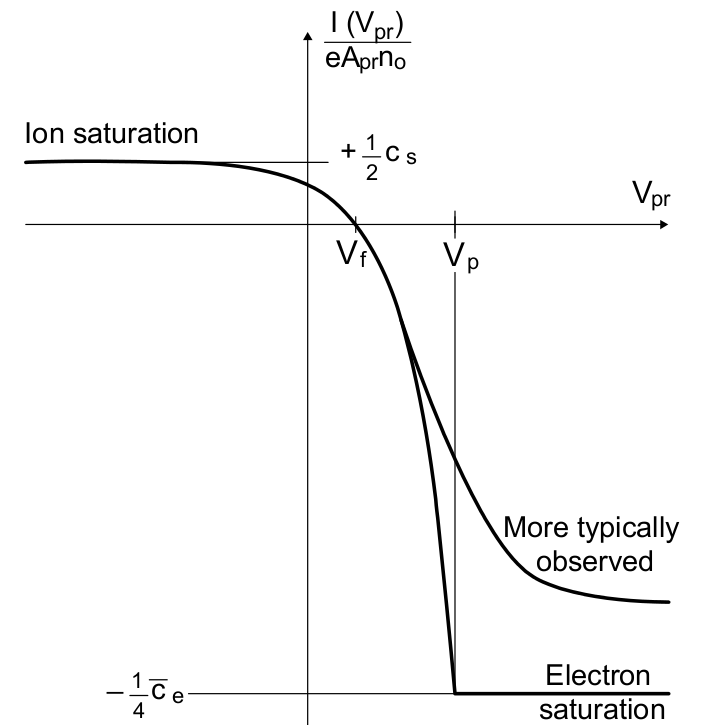
\includegraphics[width=0.5\textwidth]{monkiv}
\caption{A schematic of the IV curve obtained with a single Langmuir probe \cite{monk}. The first curve is what is expected in the ideal case where as the second curve shows what is more likely to be seen in an experiment}
\label{circuit}
\end{figure}
The electron temperature can be determined by the gradient of the IV curve where as the ion saturation current gives the electron density. Experiment has shown that IV curves obtained in practise differ from those predicted by theory in an ideal case which leads to complications in interpretation. The deviations from the ideal case are even more apparent when magnetic fields are included. 
%Probes as well as other diagnostics are used at the edge of tokamaks and other fusion devices to make measurements of the plasma conditions. Divertors are required at the edge of the tokamak in order to remove helium ash produced from fusion and other impurities that have entered the plasma from the edge of the vessel. The future success of fusion depends on the development of more advanced divertor schemes that can take out the plasma impurities and withstand the high heat fluxes long enough to make the machine economically viable. The development of more sophisticated divertors requires an improved understanding of plasma transport inside the tokamak. Probes provide boundary conditions for simulation codes that are essential to improving our understanding of plasma transport. If the data from probes is not correctly interpreted it has a knock on effect on everything else. 

\subsection{Probes in Magnetised Plasmas}
Fusion devices such as tokamaks use strong magnetic fields to confine the plasma long enough for fusion to occur. The presence of a magnetic field changes the dynamics of particles moving in the sheath and so has an impact on measurements made by probes. There is also a new region to consider the magnetic presheath. Particle transport to the probe is now restricted by cross-field diffusion and the size of the probe starts to become important. The extent of how how probe measurements are affected by the addition of a magnetic field depends on the relative size of the probe dimension $d$ to that of the Larmor radius ($r_L$) given by
\be 
r_L = \frac{v m}{e B}
\ee
Where $v$ is the velocity of the charged particle, $m$ its mass, $e$ the charge and $B$ the strength of the magnetic field in Tesla. Due to their lower mass the electrons have a much smaller Larmor radius than the ions and so are affected more by the presence of a magnetic field. Probes in tokamaks are often operated in the strong-field regime. This is defined at the point at which
\be
d > r_{L,ion} >  r_{L, electron}
\ee
The motion of both electrons and ions is strongly affected by the field. The high temperatures in the edge tokamak region place a constraint on the size of the probes as they need to be large enough to dissipate the heat and avoid being melted, so making the probes smaller in order to simplify probe interpretation is not a viable option.
In the strong field regime particles are only able to reach the probe from the direction parallel to the field so it appears to them that the probe has a plane geometry regardless of its actual geometry. This means the effective collection area of the probe is now reduced from its actual surface area to the projection of the surface in the direction of the field.  Experiments were carried out by Brown in a linear plasma device that contained two sets of diagnostics capable of measuring the electron density, Langmuir probes and a microwave interferometer \cite{probe-response}. Both diagnostics were used simultaneously while the magnetic field strength was increased. As the field became stronger the electron density derived from probe readings deviated from those obtained by the interferometry. The probes were giving a lower value of $n_e$. This can be explained by a reduction in the collection area of the probe due to the increased field which then results in a lower value for the ion saturation current ($I_{sat}^+$) and so is consistent with theory. Similar effects have been observed in fusion devices such as the DITE tokamak where Stangeby observed an uncertainty in the effective area for Langmuir probes during ion collection \cite{dite}. Stangeby also observed a discrepancy in the measured electron temperature on the DIII-D tokamak when comparing the results of the divertor Thomson scattering system to that of the Langmuir probes \cite{d3d}.
Charged particles will only be collected by the probe if their field line ends on the probe itself, so flow to the probe is dominated by cross-field transport processes which allow charged particles to move from one field line to another. The probe drains the plasma from the field lines it intercepts and further particles can only be collected if they diffuse across field lines.The most striking evidence that magnetic fields affect probe readings is from observing a dramatic reduction in the electron saturation current to ion saturation current ratio. Bohm predicted values as low as 10 \cite{discharges} and this was confirmed experimentally by Sugawara \cite{monk}. The electron saturation to ion saturation current ratio is now  typically $\approx$ 10 rather than $\sqrt{\frac{m_i}{m_e}} \approx 60$ as in the zero field case for a deuterium plasma.  Values for this ratio have been recorded in tokamaks to be even as low as unity \cite{matthews}. 

In order to survive the extreme heat conditions inside a tokamak fast reciprocating probes (RCP's) are used that are able to be quickly inserted into the plasma, take a measurement and are then withdrawn before over-heating. Another technique used in tokamaks is to flush mount probes into the tiles of divertor targets and limiters where they can measure the plasma parameters at the plasma surface interface. Many probes placed in arrays are able to measure profiles across the entire divertor without moving the plasma.  This set up increases the area over which the heat from the plasma is spread across the probe as the magnetic field is at grazing incidence to the probe. Also when built in to the vessel structures like this they do not perturb the edge plasma as the probe is indinguishable from the tile \cite{stangeby-2000}. The typical angle between the magnetic field and the divertor tile is $\approx 7 ^{\circ}$ but can be as low as $1^{\circ} \to 2^{\circ}$.  Unfortunately these advantages come at a cost, flush mounted probes are even harder to interpret than probes at normal incidence to the magnetic field. 
 
Let $\theta$ be the angle between the field and the normal to the probe surface as shown in figure \ref{fig:angle}. The electron density is obtained using the ion saturation current 
\be
ne = \frac{I^+_{sat}}{V_B A e} 
\ee
Where $A$ is the projected area of the probe normal to the field and $V_B$ the voltage applied to the probe. For flush mounted probes it is assumed $A = A_s cos(\theta)$ where $A_s$ is the exposed geometric area of the probe and $\theta$ is the angle between the normal to the surface and $\vec{B}$. This assumption comes from the fact that the parallel velocity of ions at the surface is roughly 2 orders of magnitude greater than the cross-field velocity. It is assumed that this relation holds up to angles greater than $89 ^{\circ}$ but this should break down once particle flow to the probe becomes dominated by anomalous cross-field transport. Experiments were carried out at the DITE tokamak in the early 1990's to test the $cos(\theta)$ relationship and determine an angle for which it broke down. 
\begin{figure}[H]
\centering
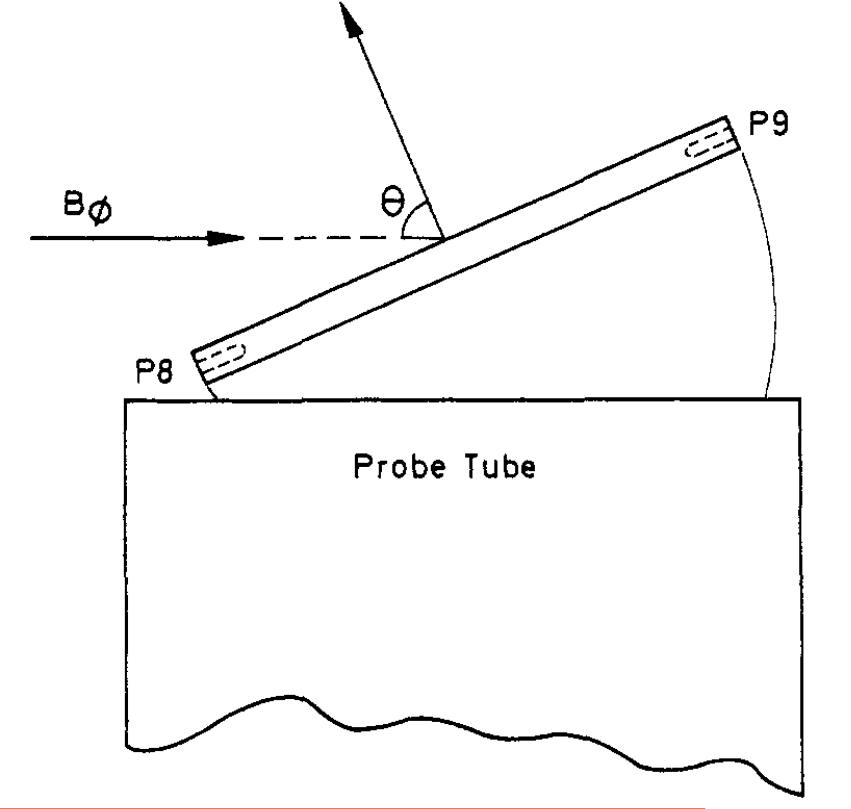
\includegraphics[width=0.5\textwidth]{angle}
\caption{A diagram of the tilting probe array. In the experiment it was possible to vary the angle between the field and the array. \cite{tilting}}
\label{fig:angle}
\end{figure}
Figure \ref{fig:angle} shows the tilting probe array (TPA) used in the DITE tokamak. The TPA had seven Langmuir probes flush mounted to the front surface and was able to be tilted to change the angle between the magnetic field and the probes. IV curves were plotted at each angle to see what impact this would have on probe readings. A selection of these IV curves are shown below. 
\begin{figure}[H]
\centering
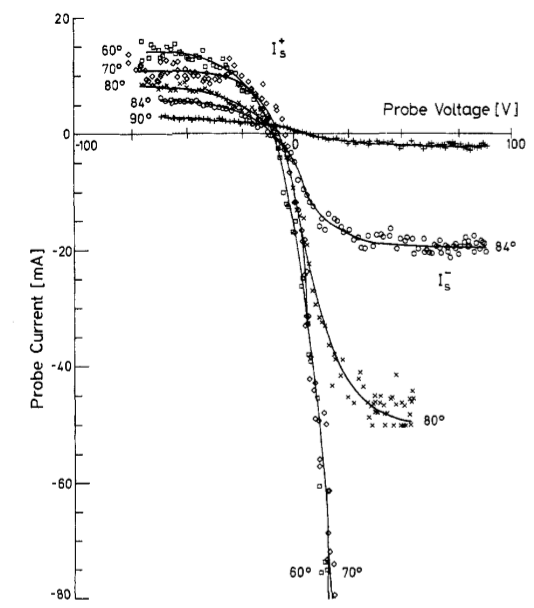
\includegraphics[width=0.5\textwidth]{lpangle}
\caption{IV curves obtained on the DITE tokamak using a tilting probe array as a function of $\theta$.  \cite{tilting}}
\end{figure}
At $90^{\circ}$ the magnetic field is parallel to the surface of the TPA. Both saturation currents decrease as $\theta \to 90^{\circ}$ as cross-field transport begins to become the dominate process for particle transport to the probe. The electron current drops faster than the ion current as angle is increased, again demonstrating how the electron side of the curve is more effected by the presence of the magnetic field. It is necessary to spread the heat load over as large an area as possible in the divertor in order to reduce damage to the surface material and reduce contamination of the core plasma, it is therefore desired to maximise $\theta$ in order to  maximise the surface area. Experiments with the TPA showed that the ion saturation no longer saturated once $\theta = 90 ^{\circ}$ but instead increased approximately linearly with applied voltage to the probe. At this angle the ratio of electron to ion saturation was also unity. This further complicates interpretation of data as a value for ion saturation current is required to extract the plasma density. It has been suggested by Carlson that the non saturation of the ion current is due to sheath expansion effectively increasing the collection area of the probe. For a flush mounted probe the sheath thickness is comparable to the size of the projected area of the probe. 
In summary the experiments using the TPA
showed that: \\
\\
1) The ratio of $\frac{I_{sat}}{E_{sat}}$ is a  strong function of $\theta$\\
2) $I_{sat}$ no longer saturates at small $\theta$ and
increases approximately linearly with applied voltage to the probe \\
3) The fitted electron temperature is too high for flush mounted probes\\ 

Probe interpretation in magnetised plasmas is clearly complex and further complicated by the presence of secondary electron emission, negative ions and collisions with neutrals. No theoretical model is capable of converting probe measurements into plasma parameters that are consistent with other diagnostics over a large range of operating parameters. The electron current is strongly distorted by the presence of a magnetic field as demonstrated by the low electron saturation current observed in experiments. The electron saturation region is not often used in experiments as the high particle flux would cause the probe to melt and so it may appear as though a low saturation current isn't really a problem. However it has been shown in JET that the electron current increases more slowly than expected for all points above the floating potential. This means that as more points are included from the region of net electron collection the value of the derived electron temperature increases. For RCP's it may be possible to limit analysis of probe data to just that collected below the floating potential where the probe is predominately collecting ions which are relatively unaffected by presence of a magnetic field. However by doing this the derived electron temperature is based only on the high energy tail of the electron distribution which is capable of reaching the negative probe, if this distribution isn't Maxwellian the electron temperature will be overestimated. It is also sometimes necessary to include points from the electron collection region when dealing with noisy data otherwise statistical noise begins to dominate the results.

The aim of my project is to develop a code capable of numerically simulating the behaviour of a Langmuir probe in a magnetised plasma. Unlike experiment, simulation provides the capability for perfect diagnostics as the energy distributions and densities of particles can be calculated without perturbing the plasma. By accurately reproducing the behaviour of a probe via simulation it will be possible to generate IV curves when the plasma parameters are already known. Experimental IV curves can then be compared to ones in the simulation database in order to extract the plasma parameters. The main aims of my project are summarised below. \\
1) To produce a generic code valuable to Fusion and Technological plasma communities that model the charged particle collection in a variety of magnetic fields, plasma environments and with a range of  probe geometries.\\
2) To produce a code/model that can predict the probe I-V characteristic for a given set of plasma operating parameters and probe geometries. The model will provide confidence in obtaining the “true”  local plasma parameters from  fitting measured characteristics to those in the model database.\\
3)The model/simulation will be user-friendly and have a user interface. \\
4)The model will be ideal for interpreting flush mounted probe data obtained in the new Super-X divertor of MAST\\
5) The model will be applied to Langmuir probe data obtained on the Liverpool Magnetron rig. 

The type of code I will be using is called a Particle-In-Cell (PIC) code that is a form of kinetic simulation. PIC codes are considered to be the most fundamental way to model a plasma short of modelling all $\approx 10^{20}$ particles. Individual electrons and ions are tracked as they move through phase space, their positions and velocities are updated at each time step by calculating the force acting on each particle and solving the equations of motion. In comparison to fluid codes, PIC codes are computationally expensive  and take large amounts of time to run. However fluid codes assume a Maxwellian velocity distribution of particles which is not a realistic assumption to make in the sheath region.

PIC simulations have been applied to probes in an attempt to understand anomalous behaviour. The SPICE3 code which is fully 3d-3v was used to understand the behaviour of the Katsumata probe. The unexpected behaviour was explained by the presence of an EXB drift that simulations revealed but was not predicted from theory \cite{SPICE3}. Another PIC code XOOPIC has been applied to study the distribution of ion flux in the tunnel of a tunnel probe on the CASTOR tokamak \cite{CASTOR}. My project aims to build on this work by providing a general code applicable to many probe geometries and will also include plasma-surface interactions such as secondary electron emission and sputtering which has not been considered in other codes. In order to gain an understanding of PIC codes I have written my own in the C language. This is a one dimensional code and will not be the main code used for the duration of my project. The main code used will be an already established but yet to be decided three dimensional PIC code. This report will now detail the basic PIC algorithm before moving on to discuss my code in more detail.

\section{Particle-In-Cell Methods}
PIC simulations track the position and velocity of all the particles in the simulation domain. Particles are given an initial position and velocity which is then updated at each time step based on the forces acting on the particle. I have developed a one dimensional code and so only one dimensional problems will be considered in this report. However PIC codes are used to model fully three dimensional problems and I will be using a three dimensional code for the majority of my project. In the one dimensional case particles are free to move over a continuous domain of length $L$ and can take any position between 0 and $L$. Plasma particles interact with each other via direct collisions and electrostatic forces. To calculate the forces acting on each particle due to every other particle present in the system would be far too computationally expensive when there are large numbers of particles present such is the case in plasma simulations. To make the simulations computationally feasible PIC codes discretise the domain into a grid as shown below.
\begin{figure}[H]
\centering
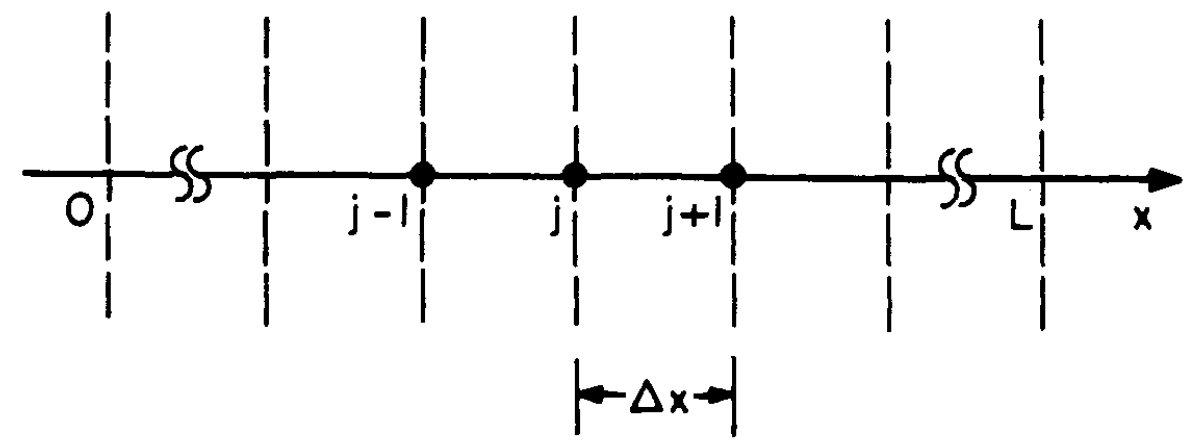
\includegraphics[width=0.8\textwidth]{grid_1d}
\caption{A representation of the one dimensional grid on which charge densities and fields are calculated. In the case of a uniform grid the grid spacing is $\Delta x$. \cite{bible}}
\label{fig:Leapfrog}
\end{figure}

The grid is a mathematical construct that makes it possible to solve differential equations such as Newton's equations of motion and Poisson's equation for the electrostatic potential. It also allows particles to interact with each other via a charge density rather than having to calculate the force between every pair of particles and so greatly reduces the run time of simulations. Splitting a physical, continuous domain  up into grid cells does have implications which need to be considered in order to ensure the simulation can still produce physically accurate results.

A PIC simulation follows an algorithm that starts with weighting the charge density of particles on to each grid point, typically particles will contribute charge only to the grid points closest to them. Once the charge density has been calculated it is then used to work out the electric potential by solving Poisson's equation. Again the potential is only solved at each grid point. Potential values are now used to calculate electric field values at the grid points which are then interpolated back to the particles, typically using the same weighting as for charge density so that new particle velocities and positions can be determined. Once the particles have been moved, the PIC algorithm is complete, time is advanced by one time step and the whole cycle repeats with a new density being calculated based on the new positions of the particles. This cycle will carry on until a certain time has been reached or steady-state has been obtained. PIC simulations are restricted by the size of the grid cells and the value of the time step.
\begin{figure}[H]
\centering
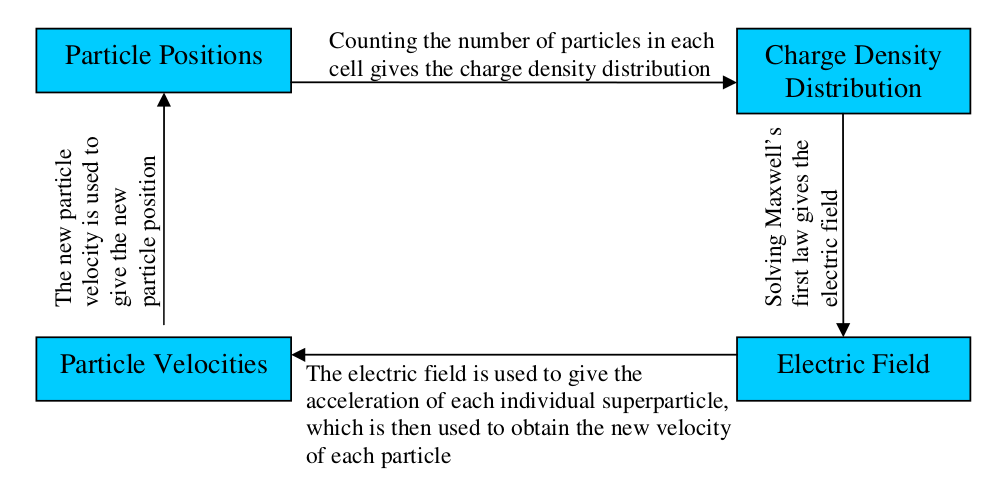
\includegraphics[width=0.8\textwidth]{piccycle}
\caption{A flow chart of the PIC algorithm \cite{loop}}
\label{fig:Leapfrog}
\end{figure}

\subsubsection{Calculating the Density}
As discussed before particles are free to take any position along the domain and their positions determine the amount of charge they contribute to the grid points nearest them. Different weighting schemes can be used, some more accurate(less noisy) than others but at the expense of longer computation time. Weighting is the name given to how the charge density on the discrete grid points is distributed and also how the force exerted on the particles from the grid points is then calculated. 
First order weighting also known as the Cloud In Cell (CIC) method is commonly used as it smooths the density and field fluctuations adequately without being too slow. In this method each particle contributes charge to its nearest two grid points. The first step calculates the offset of the particle from the closest grid point to its left. 
\be
offset = x_i - X_j 
\ee 
where $x_i$ is the particles position and $X_j$ the grid point. $x_i > X_j$ always. The charge assigned to the $J^{th}$ grid point is then 
\be 
q_j = q_c \left(1 - offset\right)
\ee 
where $q_c$ is the charge of the particle. 
The charge assigned to the J+1 cell is 
\be 
q_{j+1} = q_c \left(offset\right)
\ee 
The weighting puts the fraction of the clouds charge which is in the $J^{th}$ cell to the $X_J$ grid point and the rest of it goes to the $X_{J+1}$ grid point. This  gives the particle a triangular shape, so the particle is effectively a triangular cloud of uniform charge centred at $x_i$ with a width of $2\Delta x$ as it is able to influence a grid point from both sides of it. 
\begin{figure}[H]
\centering
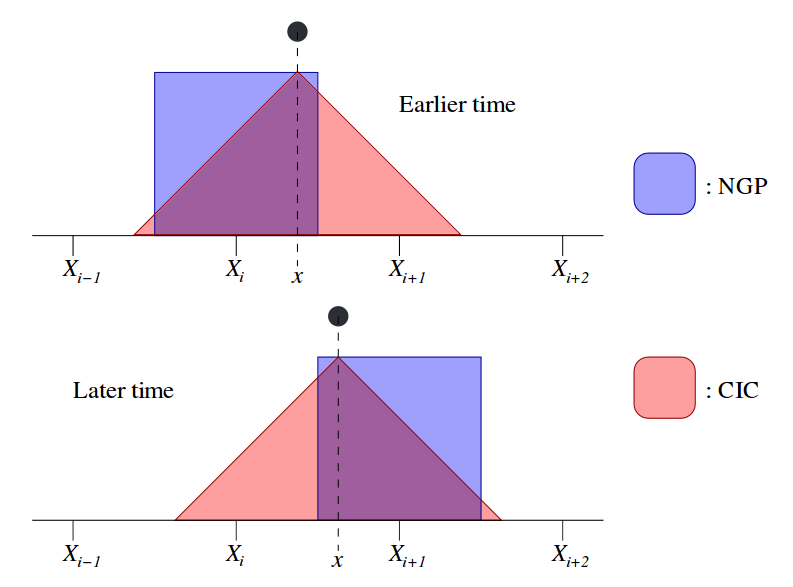
\includegraphics[width=0.8\textwidth]{particleshape}
\caption{The effective shape of a particle at position x as seen by the grid.\cite{shape}}
\label{fig:shape}
\end{figure}

\subsubsection{Calculating the Potential}
The potential can now be calculated from the known charge density at every grid point by solving Poisson's equation
\be
\frac{d^2 \psi}{dx^2} = \frac{e}{\epsilon_0} (n_e - n_i)
\ee 

This can be solved numerically by a computer using the Finite Difference Method (FDM). FDM solves differential equations via the discretisation of its derivatives. 
In FDM the solution to the equation is only known at the grid points, the potential is no longer a continuous function. Combining the forward difference and backward difference solution like this is known as central differencing and is second order accurate.
\be 
\frac{{\partial}^2\psi}{\partial x^2} = \frac{\psi_{j+1} -2\psi_{j} + \psi_{j-1}}{{(\Delta x)}^2} = -\frac{\rho_j}{\epsilon_0}
\label{eq:phisolver1}
\ee 
The value of $\psi$ at grid point j, ($\psi_j$),  depends on the value of $\psi$ at the two grid points either side of it $(\psi_{j-1}$ and $\psi_{j+1})$, so the grid points are coupled together. In order to find the value of $\psi_j$ at $N$ different grid points requires the solution of $N$ coupled linear equations. 


These coupled equations can be expressed in matrix form. 
\be
\begin{pmatrix}
  B_{1} & C_{1}  \\
  A_{2} & B_{2} & C_2 \\
        & A_3  & B_3 & C_3   \\
        & & \ddots & \ddots & \ddots \\
        & & &  A_N & B_N
\end{pmatrix}
\begin{pmatrix} 
 \psi_1  \\ 
 \psi_2  \\ 
 \psi_3  \\ 
 \vdots  \\
 \psi_N
\end{pmatrix}
= 
\begin{pmatrix} 
 \rho_1  \\ 
 \rho_2  \\ 
 \rho_3  \\ 
 \vdots  \\
 \rho_N
\end{pmatrix}
\ee
Where $A=1, B=-2$ and $C=1$.  This matrix equation must now be solved in order to obtain the potential at each grid point. Plenty of matrix solvers exist including the tridag solver found in Numerical Recipes \cite{NumericalRecipes}. 
\subsubsection{Calculating the Electric Field}
Once the potential is known at each grid point the electric field is easily found by calculating the gradient of the potential.
\be 
E = - \nabla \psi
\ee 
which in one dimension becomes
\be 
E = - \frac{\partial \psi}{\partial x}
\label{eq:electricfield}
\ee
This can discretised as before becoming
\be 
E_J = - \frac{\psi_{J+1} - \psi_{J-1}}{2 \Delta x}
\ee 
and at the boundaries 
\be
E_0 = \frac{3\psi_0 + \psi_2 - 4\psi_1}{2\Delta x}
\ee 
The exact same method in the backwards direction gives 
\be 
E_N = \frac{4\psi_{N-1} - \psi_{N-2} - 3\psi_N}{2\Delta x}
\ee 

\subsubsection{The Particle Mover}
The final step in the PIC cycle is to move the particles which requires calculating a new position and velocity for each particle in the simulation based on the forces acting on them. In order to do this Newtons equations of motion must be solved 
\be 
\vec{F}  = m \frac{d \vec{v}}{d t}
\ee 
\be 
\vec{v} = \frac{d \vec{x}}{d t}
\label{eq:diff2}
\ee 

Ignoring the presence of a magnetic field for now and limiting to one dimension gives the following equation of motion.
\be 
\frac{d \vec{v(x)}}{d t} = \frac{q}{m} E(x)
\label{eq:diff1}
\ee

The particles positions and velocities can be found by integrating the differential equations \eqref{eq:diff2} and \eqref{eq:diff1}. Many integration methods exist, the leap-frog method is commonly used due to its accuracy, stability and computational ease \cite{second_order}. Instead of using the velocity at the beginning of the time step to advance the position it uses an average value of velocity throughout the time step. The leap-frog method involves offsetting the velocity by half a time step from the position. So the velocity of the particles is only known at half integer time steps while the positions are known at integer time steps. 
\be 
v_{t+1/2} = v_{t- 1/2} + \frac{qE_t}{m} \Delta t
\ee
\be 
x_{t+1} = x_{t} + v_{t+1/2} \Delta t
\ee 
This requires the initial velocities of the particles to be moved back half a time step at the beginning of the simulation, a "de-acceleration", in order to have time centred velocities. This just requires calculating the fields as before. This method is known as Leap-frog because in order to calculate new positions requires a leap over the known velocity. 

\begin{figure}[H]
\centering
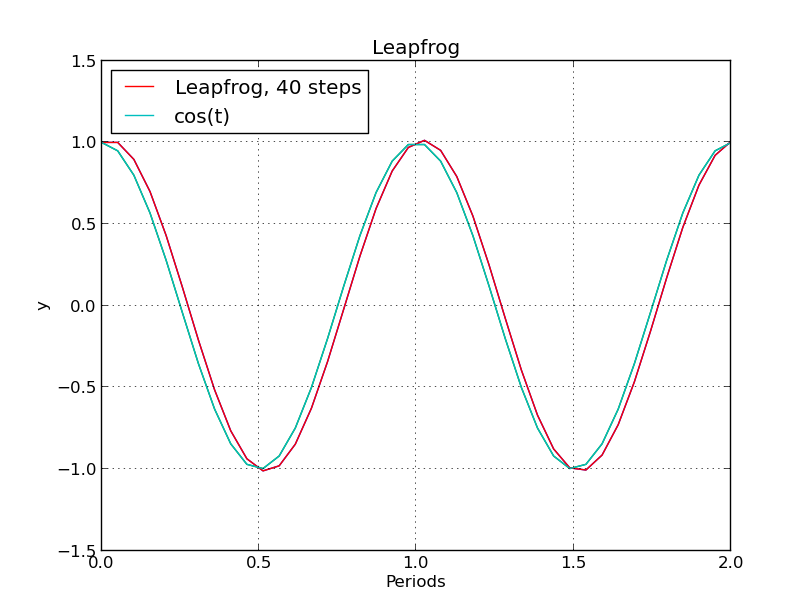
\includegraphics[width=0.8\textwidth]{Leapfrog}
\caption{A graphical representation of the Leap-Frog scheme\cite{shape}}
\label{fig:Leapfrog}
\end{figure}
In order to develop an understanding of PIC codes I have developed my own code which I have tested and benchmarked against the well established Berkeley code XES1 to ensure it is working correctly. The code required for my project will need to be fully three dimensional, with collisions and many other physics that I have not had time to put in my code. The code I have developed is not the one I will be using for the duration of my project but it will provide a test bed for new physics to test code changes quickly before editing the larger, more complex code. 

\section{Testing My Code}
I have developed a code with periodic boundary conditions in order to allow benchmarking comparisons to be made with XES1. I have also made a code capable of simulating the behaviour of a floating wall in front of a plasma. The floating case is very similar to the type of problem I will encounter whilst simulating probe behaviour. The periodic results will be discussed first before moving on to the floating case. 
\subsubsection{Cold Plasma Oscillations} 
It is well known that if electrons in a plasma are displaced from their equilibrium position they will feel a restoring force due to electric fields which will act to quickly return the electrons to their equilibrium position. Once they reach this equilibrium position their kinetic energy will cause the electrons to overshoot and so a cycle begins with electrons oscillating around their respective equilibrium positions. The time frequency at which these oscillations occur is called the plasma frequency ($\omega_p$). This is related to fundamental plasma parameters as 
\be 
\omega_p = \frac{n_e m}{q^2 \epsilon_0} 
\ee
In a real plasma these oscillations are non-dispersive, the frequency the electrons will oscillate at is always the plasma frequency and does not depend on the initial amplitude or wave number of the displacement. This is not the case in a periodic PIC simulation of the plasma, alias effects from the grid introduce a dispersion relation. The frequency the electrons will oscillate at now has a wave number dependence \cite{bible}
\be 
\omega(k) = \omega_p cos\left(\frac{k \Delta x }{2} \right) 
\ee
$\omega(k)$ is the frequency that will be measured in PIC experiments. It is possible to measure this by plotting the kinetic energy of the electrons against time. As a first test a plot was made of kinetic energy and potential energy against time.
\begin{figure}[H]
\centering
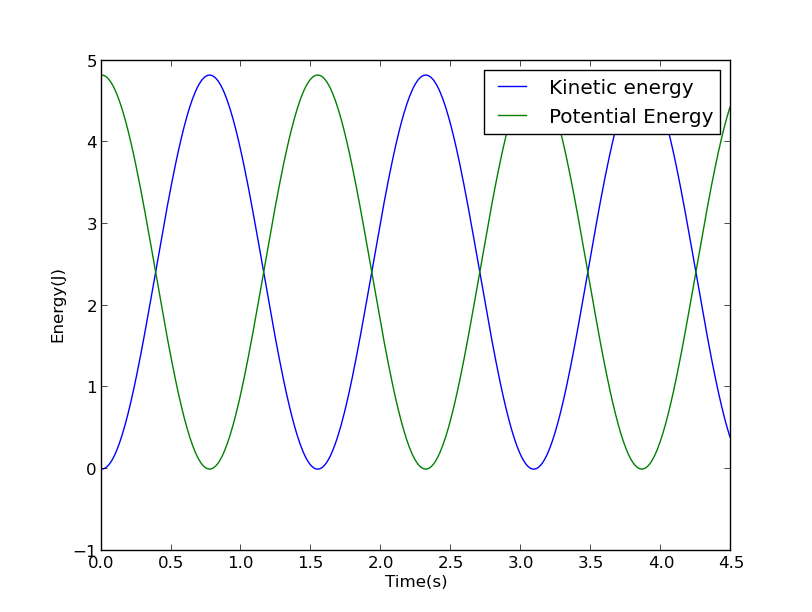
\includegraphics[height=0.5\textwidth]{keandpe.png}
\caption{A plot of Kinetic energy and Potential Energy versus time. Shows the interchange of kinetic energy with potential energy}
\end{figure}
The electrons begin stationary with no kinetic energy. Their displacement gives them a potential energy which is converted into kinetic energy. The velocity has a sinusoidal dependence of time, the kinetic energy $(\tau)$ therefore obeys 
\be 
\tau = Asin^2(\omega_p t)
\ee
where $A$ is the amplitude. By fitting this curve to the plot of kinetic energy it is possible to determine 
$\omega_p$. This can be carried out for multiple wave numbers to see if the plasma frequency does have a  mode dependence. 

The code was set up with the following parameters. 
\begin{table}[h]
\begin{tabular}{lllll}
L  & ${2\pi}$      \\
GP & 512    \\
N  & 1024   \\
W  & 1e6   
\end{tabular}
\end{table} 
The code was ran with different modes ranging from 1 to 70. The plasma frequency was measured for each and the results are shown below along with the theoretical dispersion relation.
\begin{figure}[H]
\centering
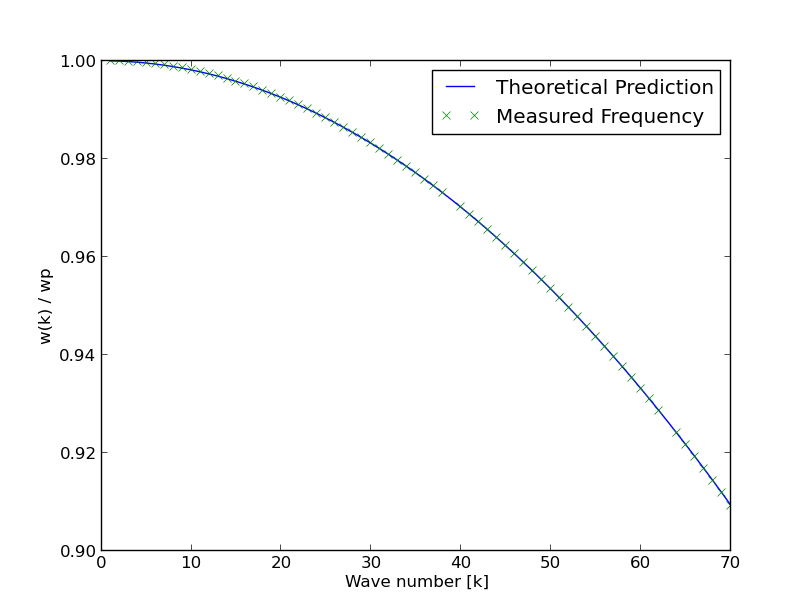
\includegraphics[width=0.8\textwidth]{cold_results.png}
\caption{Dispersion Relation for the cold plasma oscillations both measured and theoretical}
\end{figure}
The two are in good agreement with each other thus demonstrating the aliasing effects of the grid.

\subsubsection{Cold Beam Instability} 
The cold beam instability is another phenomenon found to occur in periodic PIC codes but in reality the system is stable. It is again caused by an aliasing effect from the grid. During this instability an initially cold beam of electrons will heat up until a saturation temperature is reached, at which point the instability is quenched.  The electrons are initially given a uniform drift velocity $v_0$ and are uniformly distributed throughout the grid. The instability leads to an increase in thermal energy of the particles but not at an expense of their initial kinetic energy, as a result the total energy of the system increases due to this instability which is a non-physical result. Theory predicts the instability will stop once 
\be 
\frac{\Lambda_D }{\Delta x} = \frac{v_t}{w_p \Delta x} \approx 0.046
\label{eq:cold_beam}
\ee 
The effects of the instability are shown below. 
\begin{figure}[!hbt]   
\begin{minipage}[t]{0.35\textwidth}
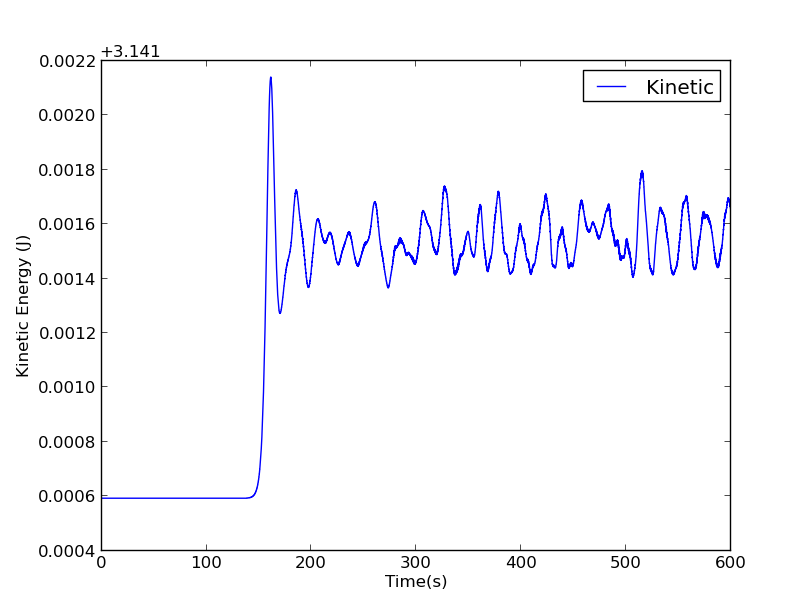
\includegraphics[width=\linewidth]{KineticEnergy.png}
\caption{The kinetic energy of the simulation increases with time until the instability saturates.}
\label{fig:immediate}
\end{minipage}
\hspace{\fill}
\begin{minipage}[t]{0.35\textwidth}
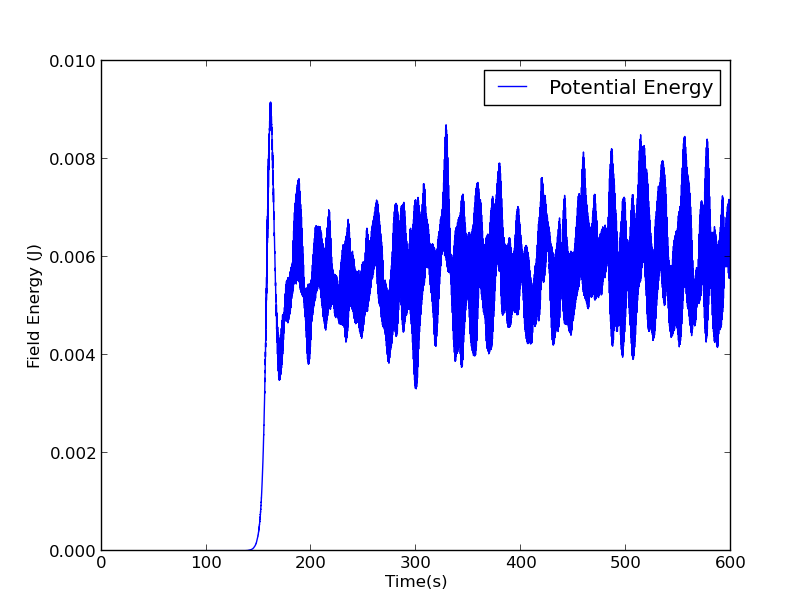
\includegraphics[width=\linewidth]{FieldEnergy.png}
\caption{The potential energy of the simulation also increases with time until the instability saturates.}
\label{fig:proximal}
\end{minipage}

\vspace*{0.5cm} % (or whatever vertical separation you prefer)
\begin{minipage}[t]{0.35\textwidth}
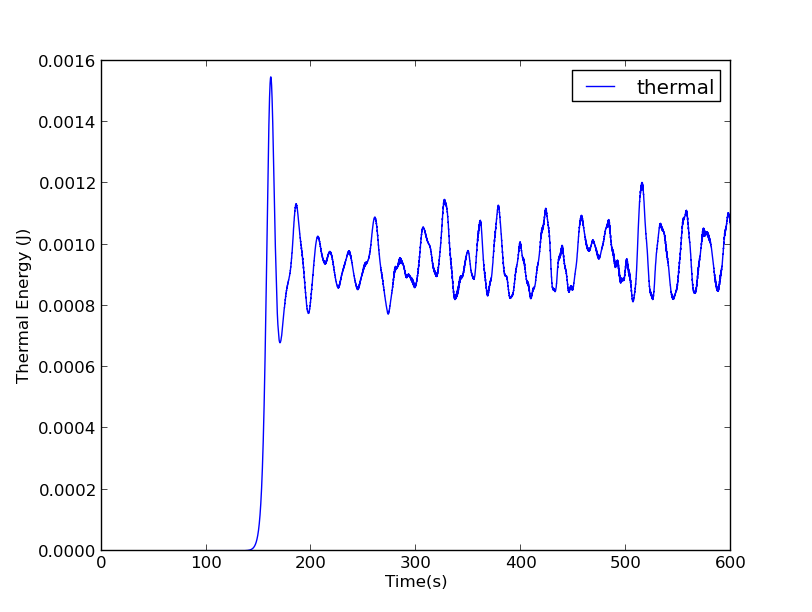
\includegraphics[width=\linewidth]{ThermalEnergy.png}
\caption{The beam gains thermal energy due to the cold beam instability. The instability saturates once the beam has warmed sufficiently}
\label{fig:distal}
\end{minipage}
\hspace{\fill}
\begin{minipage}[t]{0.35\textwidth}
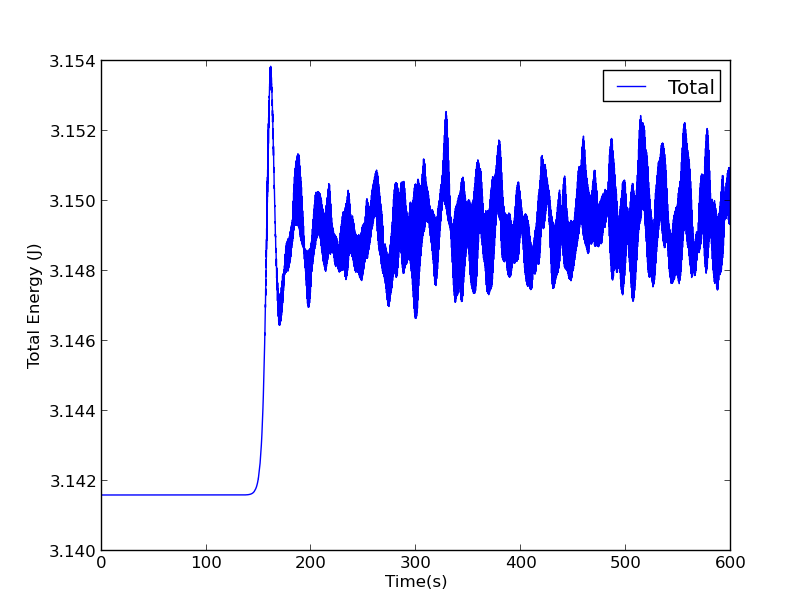
\includegraphics[width=\linewidth]{TotalEnergy.png}
\caption{The instability leads to an unphysical source of energy, it is not the initial drift energy that is converted into thermal energy. }
\label{fig:combined}
\end{minipage}

\end{figure}
\newpage
The thermal energy of the beam rises until a critical temperature has been reached, at that point the instability abruptly stops and energy fluctuates but does not grow. To test the point of saturation simulations were run with my code keeping the length of the system the same but varying the number of grid points which is equivalent to changing $\Delta x$. In all runs the length of the system was $2\pi$ and the same number of particles were used with the same initial velocity. The thermal energy at saturation was used to determine the thermal velocity and this was then compared to \eqref{eq:cold_beam}. A coefficient of 0.049 was found to be the average result which is consistent with Berkley's XES1 code. The relation is an approximate one. Tests were also carried out on how the initial velocity of the electrons affected the thermal velocity at saturation, it was found not to have an effect which is consistent with theory.

As the instability stops once the temperature has reached thousandths of an eV it is not likely that this instability will cause any problems in simulations that I will be doing, never the less this instability provided a useful test case on which to benchmark my code. Giving a temperature to the beam at the beginning of the simulation prevents the instability from occurring provided the beam temperature is higher than the saturation temperature.

\subsubsection{Two Stream Instability}
This is a classic test case for a PIC code. The code is set up with two streams of electrons moving in opposite directions through a neutralising ion background. The beams are perturbed to give a sinusoidal density perturbation. The density perturbation in one beam reinforces the density perturbation in the other beam and vice versa. This leads to an exponential rate of growth for the instability. The initial drift energy of the electrons is converted into electric field energy which then acts to scatter the particles in phase space. As a result the temperature of the beams rises. The particles become trapped in vortices. 
\begin{figure}[H]
\centering
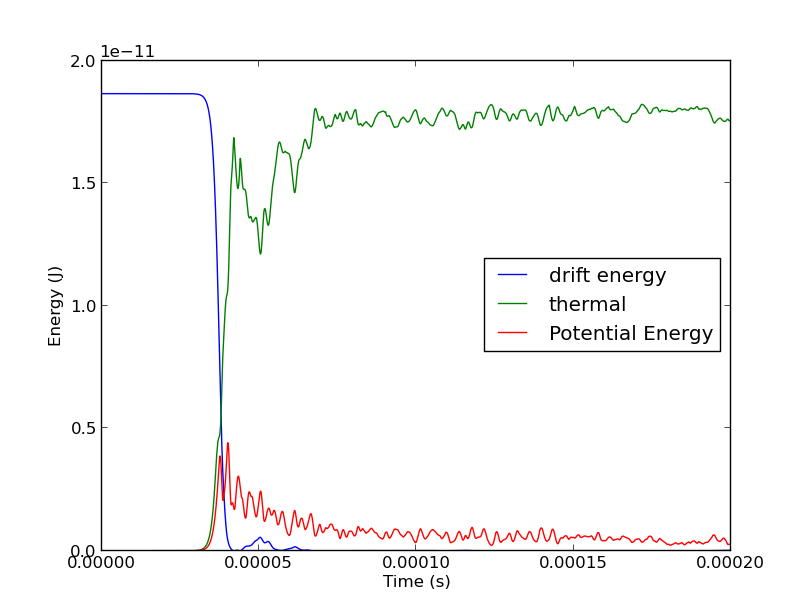
\includegraphics[width=0.5\textwidth]{all_energies_2_stream}
\caption{The initial drift energy of the beam is converted into thermal energy}
\label{fig:Leapfrog}
\end{figure}
The vortices are shown in the phase space plots below. 
\begin{figure}    
\begin{minipage}[t]{0.45\textwidth}
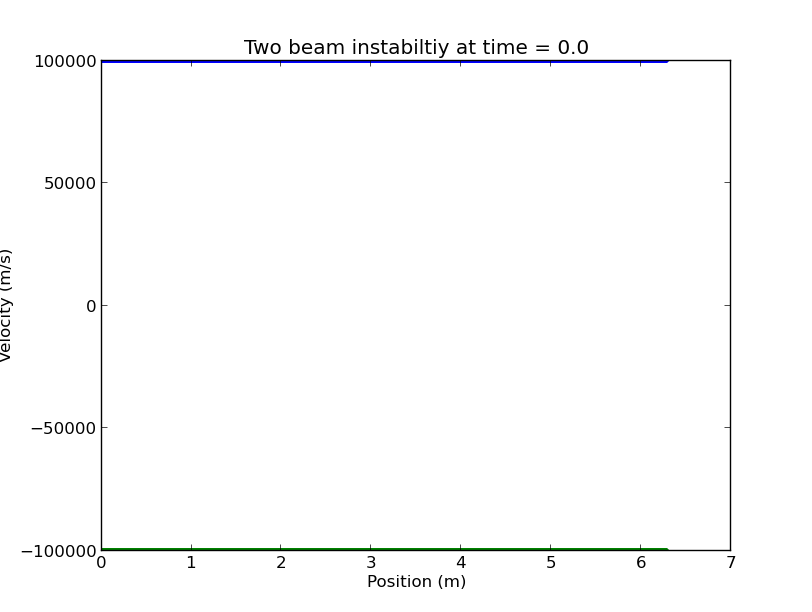
\includegraphics[width=\linewidth]{t=0.png}
\caption{Two cold beams with velocity in opposite directions.}
\label{fig:immediate}
\end{minipage}
\hspace{\fill}
\begin{minipage}[t]{0.45\textwidth}
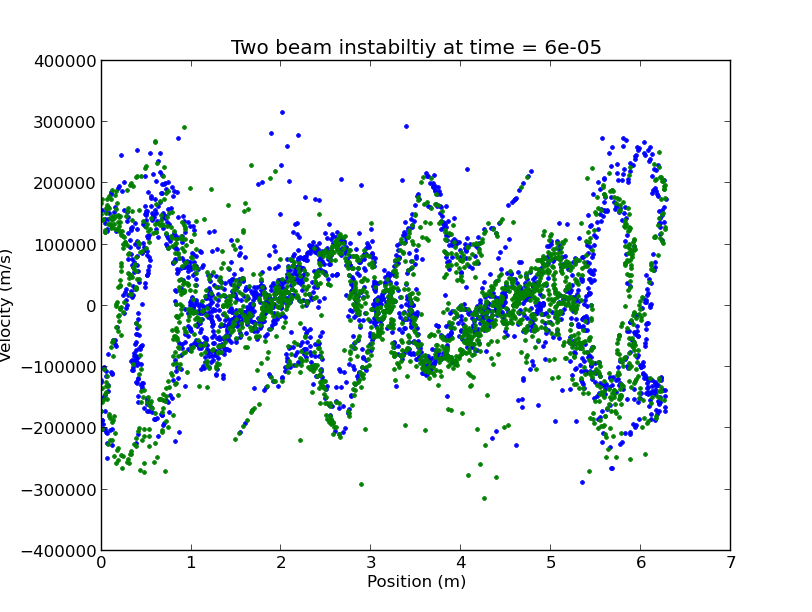
\includegraphics[width=\linewidth]{t=1.png}
\caption{Vortices form and particles begin to move backwards.}
\label{fig:proximal}
\end{minipage}

\vspace*{0.5cm} % (or whatever vertical separation you prefer)
\begin{minipage}[t]{0.45\textwidth}
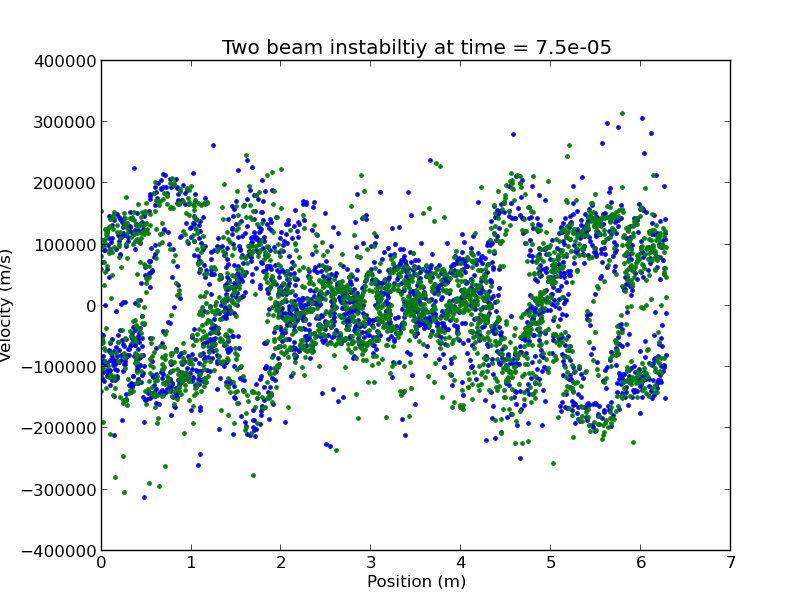
\includegraphics[width=\linewidth]{t=2.png}
\caption{Some particles gain energy up to three times their initial kinetic energy}
\label{fig:distal}
\end{minipage}
\hspace{\fill}
\begin{minipage}[t]{0.45\textwidth}
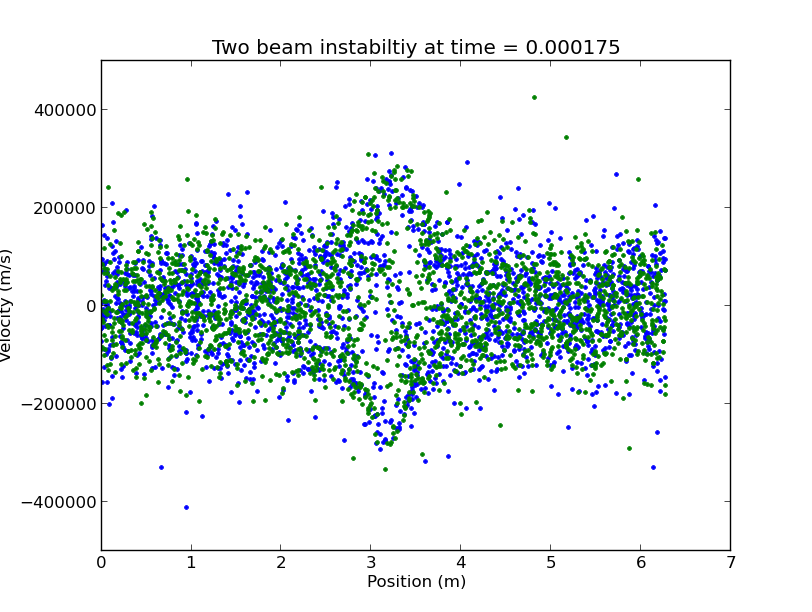
\includegraphics[width=\linewidth]{t=4.png}
\caption{The vortices eventually merge into one.}
\label{fig:combined}
\end{minipage}

\end{figure}
\subsubsection{Floating Wall} 
To make the transition from a periodic code which models an infinite plasma to a finite plasma with boundaries on either side required changing the matrix solver and adding boundary conditions. By testing my periodic code I have established every part of the code apart from the matrix solver is in working order. The matrix solver used in my code is the one provided by Numerical Recipes \cite{NumericalRecipes}. It has been benchmarked with test cases to ensure it is working correctly so I can be confident my code works as it should do. Another test of the matrix solver was the observation of a self-force, the phenomenon of a particle depositing charge on the grid and then feeling a force from that charge. This was something I investigated because it had been observed in my code but a lot of literature claims it should not exist \cite{bible} \cite{Hockney1981}. This turns out to only be the case for a periodic code and not one with boundary conditions which is misleading. More details of the self-force can be found in the appendix. 


In the floating test case a source of plasma is on the left hand side of the domain and on the right is a wall that collects the charged particles hitting it. The domain is initially filled with a uniform, neutral plasma with a temperature as specified by the user. It is possible to give the ions and electrons a different temperature. The electrons are much more mobile due to their lighter mass than the ions and so the wall quickly becomes negatively charged. This accelerates ions towards the wall and retards the flow of electrons and leads to the formation of a positive sheath in front of the wall as seen in experimental plasmas \cite{sheathformation}. At each time step equal numbers of ions and electrons are injected as pairs in the same location with a velocity sampled from a Maxwellian distribution. Injecting the particles as pairs i.e. at the same location prevents the generation of non-physical electric fields in the source region.  


\begin{figure}[H]
\centering
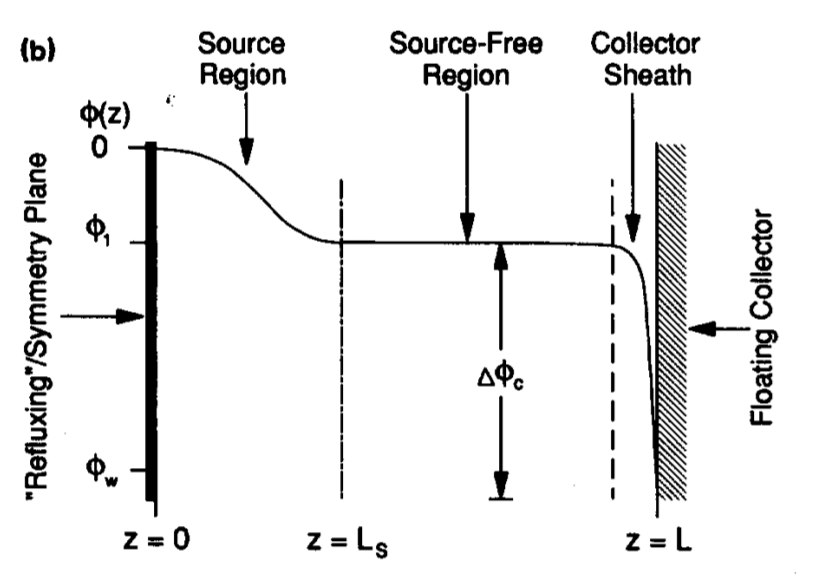
\includegraphics[width=0.8\textwidth]{float_setup}
\caption{A diagram representing the domain in the floating case. Particles are injected as pairs in the source region and travel to the wall located on the right hand side. \cite{float_diagram}}
\end{figure}



Tests were carried out to ensure the distribution of velocities is truly Maxwellian. 
\begin{figure}[H]
\centering
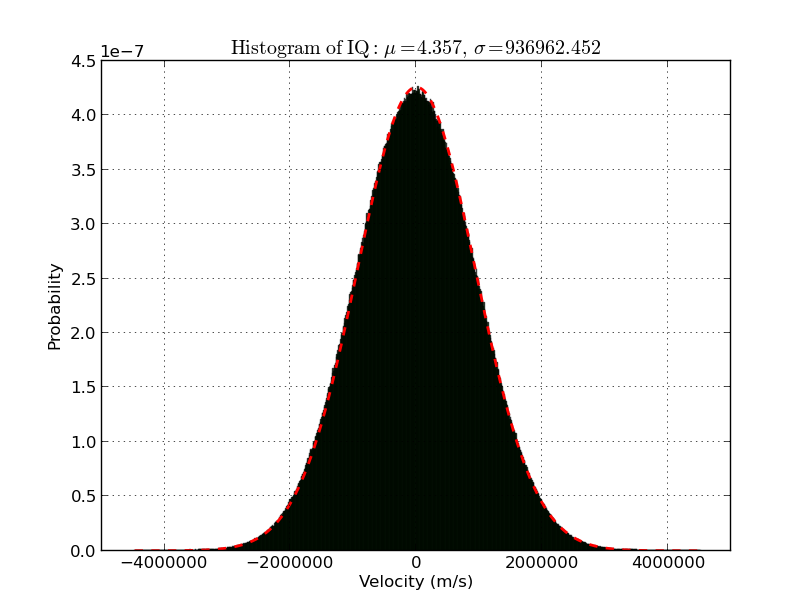
\includegraphics[width=0.8\textwidth]{maxwell.png}
\caption{The initial distribution of velocity for the electrons at 5eV.}
\end{figure}
The electrons were given a temperature of 5eV. The resulting velocity distribution has a velocity centred around zero and a standard deviation equivalent to the thermal velocity as expected.
Particles that travel across the domain and hit the wall deposit their charge on to the wall and are then deleted from the system. Particles that exit from the left hand side are refluxed. This means they are given a new velocity towards the wall sampled from a Maxwellian distribution. The idea behind this is that the source region in the code represents only a fraction of the actual source region as this will be much larger than what it is possible to simulate within a reasonable time for a PIC code. So particles that exit the domain are replaced by thermal particles travelling in the opposite direction. It is possible to reflect the particles that hit the left hand boundary rather than generate a new velocity for them, however without collisions in the model electrons that are reflected from the sheath in front of the wall become trapped in the system with a reflecting boundary on the left hand side. Refluxing provides a way to rethermalise these electrons as collisions would do.


A problem encountered with this test case is a loss of temperature in the source region. The source is initially filled with a uniform plasma at the desired temperature. However the more energetic particles quickly leave the source region and travel to the wall leaving the slower moving particles behind, lowering the temperature of the source region. The source region loses the high end energy tail of the distribution and becomes non-Maxwellian over time. Although there is a constant source of new particles it is far more likely that the new particles will be moving at a slower speed due to the nature of a Maxwellian distribution. These slow moving particles then take longer to exit the source region. This is a direct result of simulating only a small source region. To confirm that this was the source of the error and not an inherent problem in the code a test case was run in which both sides of the domain reflected particles that reached it. No particles were added to or lost from the system. In this case the temperature of the particles was the same at all times. Attempts have been made to conserve the temperature in the floating case, firstly by adding binary collisions which helps but does not remove the problem as the fast particles will still quickly escape. Other attempts involved artificially changing the velocity of all particles in the source region at a set number of time steps. Adding this feature generated electric fields in the source region which led to a rapid breakdown of the simulation. Despite this difficulty the code does exhibit physical results such as the generation of a positive sheath a few Debye lenghs wide in front of the wall and zero electric field everywhere except from the source region. These results are shown in figure \ref{fig:sheath} and \ref{fig:sheath_field}.
\begin{figure}    
\begin{minipage}[t]{0.45\textwidth}
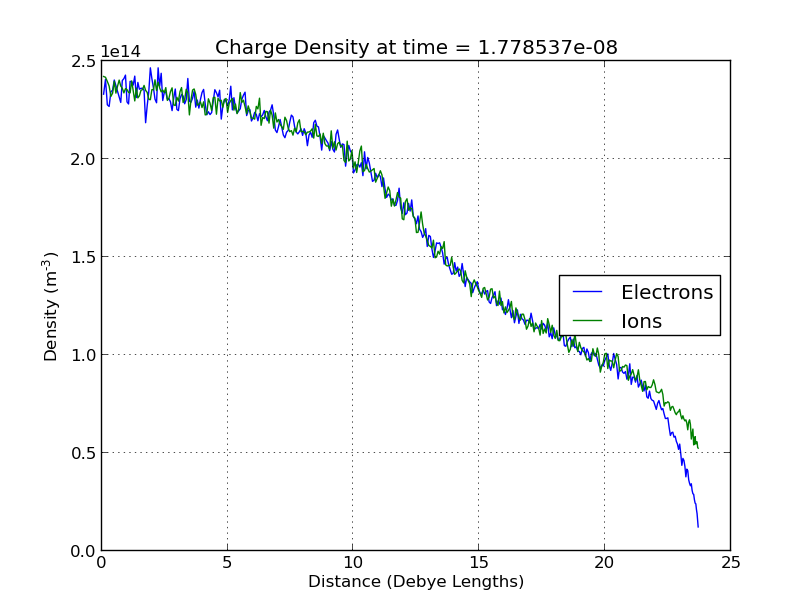
\includegraphics[width=\linewidth]{sheath_dense.png}
\caption{A positive sheath with a thickness of a few Debye length forms in front of the wall and shields the rest of the plasma from the negative charge.}
\label{fig:sheath}
\end{minipage}
\hspace{\fill}
\begin{minipage}[t]{0.45\textwidth}
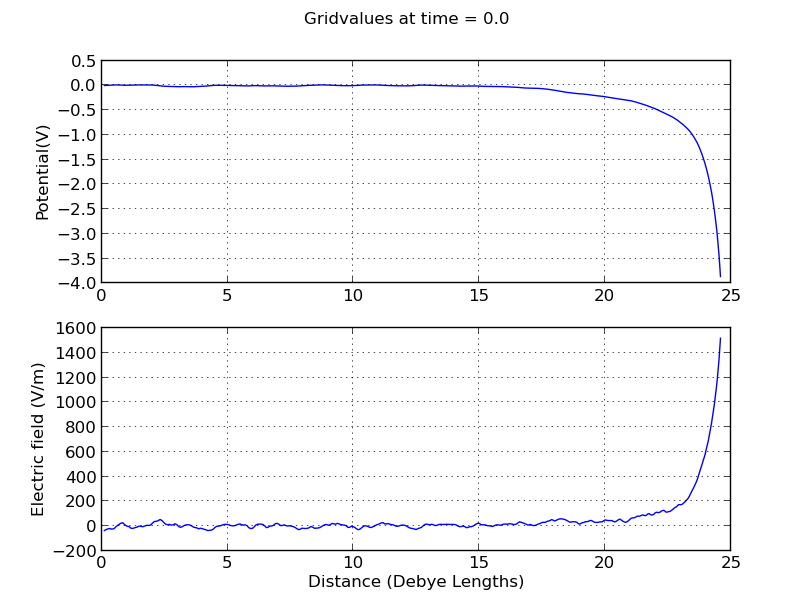
\includegraphics[width=\linewidth]{sheath_potential.png}
\caption{The electric field is zero everywhere in the quasi-neutral plasma but rapidly increases in the sheath region. This field acts to accelerate ions in the sheath and de-accelerate electrons.}
\label{fig:sheath_field}
\end{minipage}
\end{figure} 
The wall reaches a floating potential that oscillates with time. Because of the loss of temperature it is not possible to compare the floating potential with that predicted by Stangeby \cite{stangeby-2000} as this assumes a Maxwellian distribution at all times. The loss of temperature has been documented in other codes, their solution is usually to limit the time duration of the simulation to reduce the effect. Other codes such as BIT1 do manage to conserve temperature and this is a feature I will be looking for in my final code \cite{BIT1}. 



\section{Future plans}
As well as developing my own code I have also produced an extensive report discussing the PIC algorithm in detail and giving more detail into the interpretation of probes. This report will form a solid basis for an introductory chapter(s) to my thesis. My code has been tested and benchmarked against the well established XES1 code so I can be confident in the reliability of my code. The next step is to identify a 3d-3v code for use in the rest of my project. The code I have developed will provide a useful test bed to explore the effects of adding new physics before implementing it into the 3d code. A detailed plan is shown in the gantt chart below.

\begin{figure}[H]
\centering
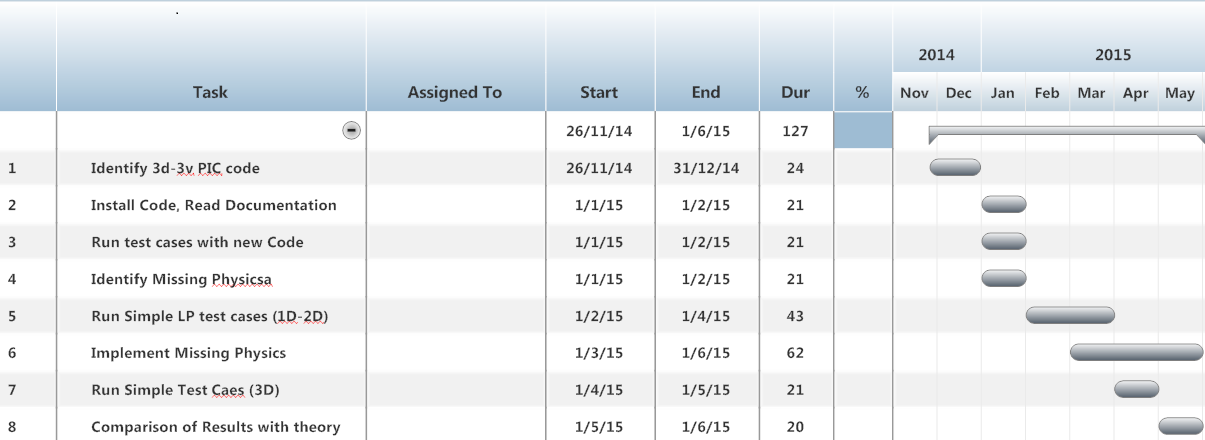
\includegraphics[width=0.8\textwidth]{plan1}
\end{figure}
Implementing missing physics from the code will be an ongoing part of my project. During this period I will also study the effects of this additional physics on Langmuir Probe data. 


\begin{figure}[H]
\centering
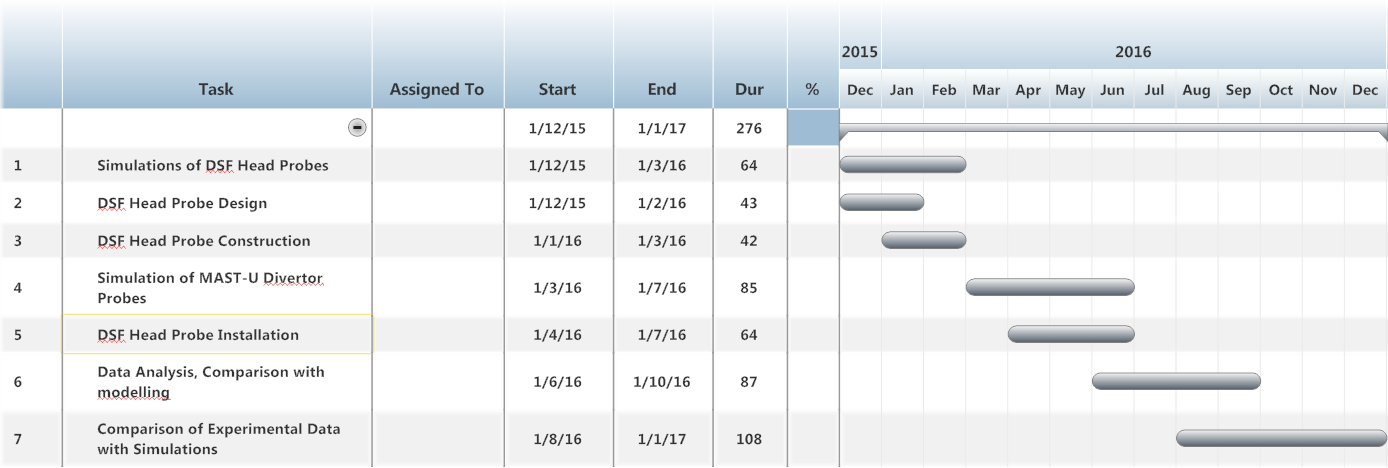
\includegraphics[width=0.8\textwidth]{plan2}
\end{figure}

The remainder of the time is scheduled for writing up.









 %https://www.google.co.uk/url?sa=t&rct=j&q=&esrc=s&source=web&cd=4&ved=0CC4QFjAD&url=https%3A%2F%2Fis.cuni.cz%2Fwebapps%2Fzzp%2Fdownload%2F140015438&ei=XmpzVJiyGdivabnKgsgO&usg=AFQjCNHm5RYgrbWnX-Z80yc0z5FsDkzqYQ&sig2=yAk37-p45aBpsnoR6gpPLw&bvm=bv.80185997,d.d2s&cad=rja

\newpage
\section{Appendix}
\subsection{Self Force}
The presence of the spatial grid introduces some non-physics into the simulation, an example of which is the self force. The self force is the name given to the phenomenon in which a charged particle becomes aware of its own field and so repels itself. This non-physical force is inherent in any system that uses the spatial grid to work out charge density and electric field values. Imagine a charged particle placed in between two grid points, let the particle reside closer to the left grid point to begin with. Using the first order weighting scheme (CIC) the particle will deposit more of its charge on to the left grid point than it will on to the right. This density will then be used to work out a potential and finally a field which is then interpolated back to the particles position, not necessarily using the same weighting scheme but for now consider it is the same. The particle will feel a larger force from the grid point on its left than it will do from the grid point on its right due to the relative distances and as a result it will be repelled from the left grid point and head towards the right. Although this argument assumed a first order weighting scheme, the self force is present with any method of weighting. 
It is possible to prove that the self force is introduced by the addition of a spatial grid rather than from any approximations made in using finite difference methods to solve Poissons equation. The following method is adapted from the textbook 'Numerical particle-in-cell Methods: Theory and Applications' \cite{selfforce}. 

The electric potential due to a point charge with charge $q$ at a distance $r$ is given by 
\be 
\psi = \frac{1}{4 \pi \epsilon_0} \frac{q}{r} = \frac{C q}{r}
\label{exact_potential}
\ee 
where $C$ is a constant. Now introduce a spatial grid with spacing $dx$. Let the particle be a distance $r$ from the grid point on the left and so a distance $dx - r$ from the point on the right. The particle will deposit a charge $\rho_1$ on the left grid point and a charge $\rho_2$ on the right where
\be 
\rho_1 = q\frac{(dx-r)}{dx}
\ee 
and
\be 
\rho_2 = q\frac{r}{dx}
\ee 
The particle will feel a potential that is a combination of the potential from the two grid points. From \eqref{exact_potential}the potential at the particle is 
\be 
\frac{C q}{dx} \left(\frac{dx - r}{r} + \frac{r}{dx - r} \right) 
\ee 
The force at the particle is given by 
\be 
F = -\frac{\partial \psi}{\partial r} q = Cq^2 dx\frac{dx-2r}{r^2(dx-r)^2}
\ee 
Despite the potential and electric field having been solved exactly without finite difference methods there still exists a self force due to the introduction of a spatial grid. This force is zero if the particle is at the midpoint of a cell ($r=\frac{dx}{2}$) and acts to repel the particle from its closest grid point.

It is possible to quantify this force in the case of a complete PIC simulation where FDM are used. As before Poisson's equation is discretised 
\be 
-\rho_J = \frac{\psi_{J+1} - 2\psi_J + \psi_{J-1}}{(dx)^2}
\ee 
This equation can be solved analytically without a matrix equation.
\be 
\psi_J = \frac{I-J}{I} A + \frac{J}{I} B + \frac{dx^2}{I} \left[(I-J) \sum\limits_{k=1}^J k\rho_k   + J \sum\limits_{k=J+1}^{I-1} (I-k)\rho_k \right]
\label{potential_analyitical}
\ee
Where $I$ is the number of the grid cells , $A$ is the potential at the left hand side boundary and $B$ the potential at the right hand side. 
This will now be carried out for one particle. Let the particle lie between grid points $x_{\alpha -1}$ and $x_\alpha$ at position $x$. The offset ($\sigma$) is given by 
\be 
\sigma = \frac{x - x_{\alpha -1}}{dx}
\ee
Using \eqref{potential_analyitical} it is possible to calculate the potential at the grid points either side of the particle. 
\be
\psi_\alpha  = \frac{I-\alpha}{I}A +\frac{\alpha}{I}B - \frac{dx^2}{I}(I-\alpha) \left[(\alpha-1)\rho_{\alpha-1} + \alpha \rho_{\alpha} \right]
\ee
\be 
\psi_{\alpha -1} = \frac{I-\alpha +1}{I}A + \frac{\alpha - 1}{I} B -\frac{dx^2}{I}(\alpha -1) \left[(I-\alpha +1)\rho_{\alpha -1} + (I-\alpha)\rho_\alpha \right] 
\ee
Similar expressions can be derived for $\psi_{\alpha+1}$ and $\psi_{\alpha-2}$. These can then be used to derive the value of the electric field at the adjacent grid points. 
\be 
E_\alpha = \frac{\psi_{\alpha -1} - \psi_{\alpha +1}}{2 dx} = \frac{A-B}{I dx} - \frac{dx}{I}\left[(\alpha -1) \rho_{\alpha -1} + (\alpha -\frac{I}{2})\rho_\alpha \right]
\ee 
\be 
E_{\alpha-1} = \frac{\psi_{\alpha -2} - \psi_\alpha}{2 dx} = \frac{A-B}{I dx} - \frac{dx}{I} \left[(\alpha-\frac{I}{2}-1) \rho_{\alpha -1} +(\alpha-I) \rho_\alpha \right] 
\ee
Using the first order weighting method, the force at the particle $E_i$ will be given by 
\be 
E_i = E_{\alpha -1 } (1-\sigma) + \sigma E_\alpha = \frac{A - B}{I dx} - \frac{dx}{I} \left[(\alpha -\frac{I}{2} -1 + \frac{I}{2} \sigma) \rho_{\alpha -1} + (\alpha -I +\frac{I}{2} \sigma) \rho_\alpha \right]
\ee
The self force is inherent in PIC codes and always acts to repel a particle from its nearest grid point going to zero when the particle is at the midpoint of a grid cell. Interestingly this equation shows the impact that boundary conditions have on the self force. The force not only depends on the location of the particle in the grid cell but also in which cell it lies in. Provided there are sufficient amount of particles the self force will be negligible.
\newpage 
\section{References}
\bibliography{references}
\end{document}
